%%%%%%%%%%%%%%%%%%%%%%%%%%%%%%%%%%%%%%%%%%%%%%%%%%%%%%%%%%%%%%%%%%%%%
%%%%%%%%%%%%%%%%%%%%%%%%%%%%%%%%%%%%%%%%%%%%%%%%%%%%%%%%%%%%%%%%%%%%%
\begin{frame}{Coupled architecture: Consensus/ Formation control}	
	\begin{figure}
		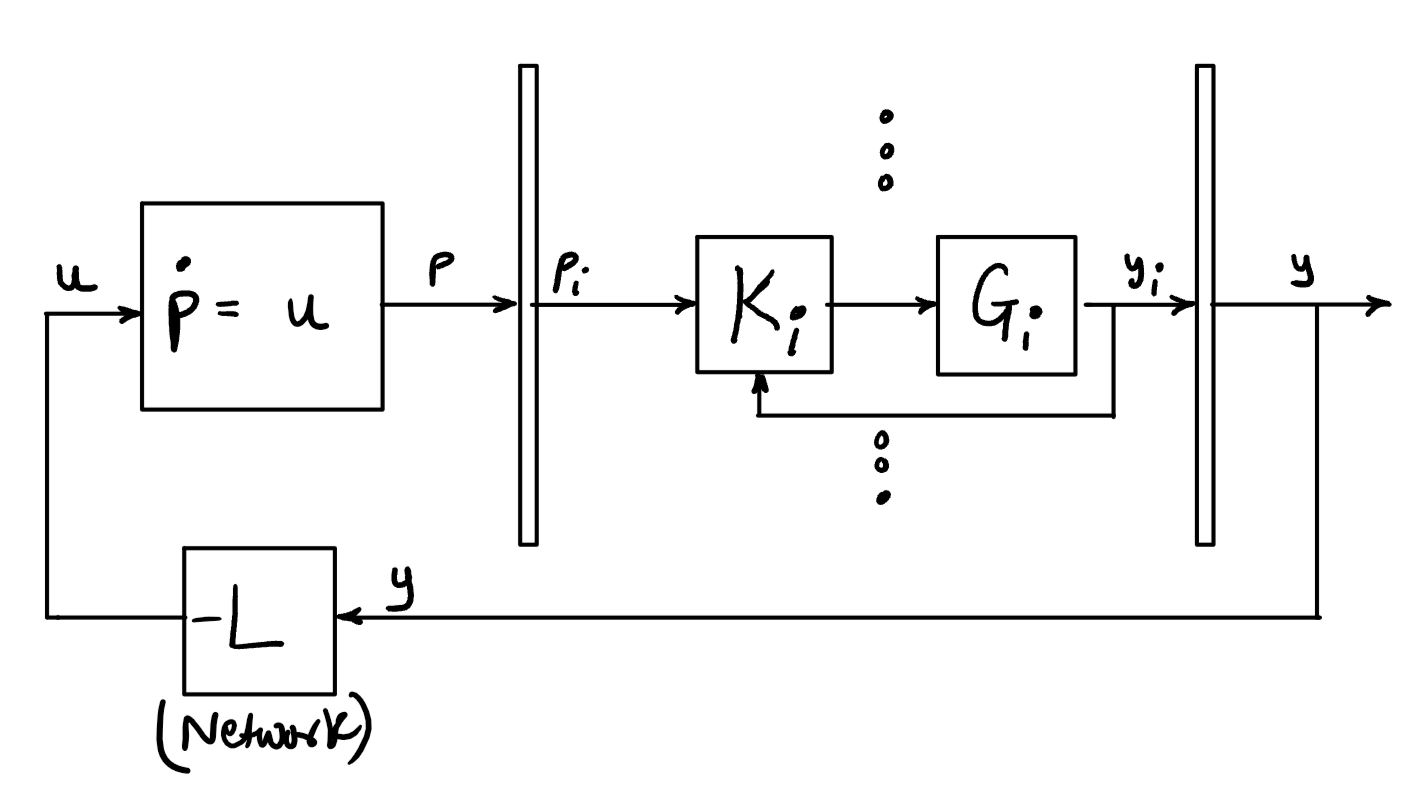
\includegraphics[scale=0.35]{figures/Coupled_consensus.jpg}	
		\label{fig:Coupled}
	\end{figure}
	\begin{itemize}
		\item Some related work
		\begin{itemize}
			\item Fixed Laplacian and LTI agents \footnote{Fax and Murray, 2004} -> Modal decomposition
			\item Fixed and uncertain Laplacian and LPV agents \footnote{Popov, 2009, Eichler and Hoffmann,2014} -> Modal decomposition 
			\item Flocking with a fixed Laplacian \footnote{B.Francis, 2016}	
			\item Interconnections of dissipative systems \footnote{M. Spong, 2006}		
		\end{itemize}
	\end{itemize}
\end{frame}
%%%%%%%%%%%%%%%%%%%%%%%%%%%%%%%%%%%%%%%%%%%%%%%%%%%%%%%%%%%%%%%%%%%%%
%%%%%%%%%%%%%%%%%%%%%%%%%%%%%%%%%%%%%%%%%%%%%%%%%%%%%%%%%%%%%%%%%%%%%
\begin{frame}{Coupled architecture: Flocking}	
	\begin{figure}
		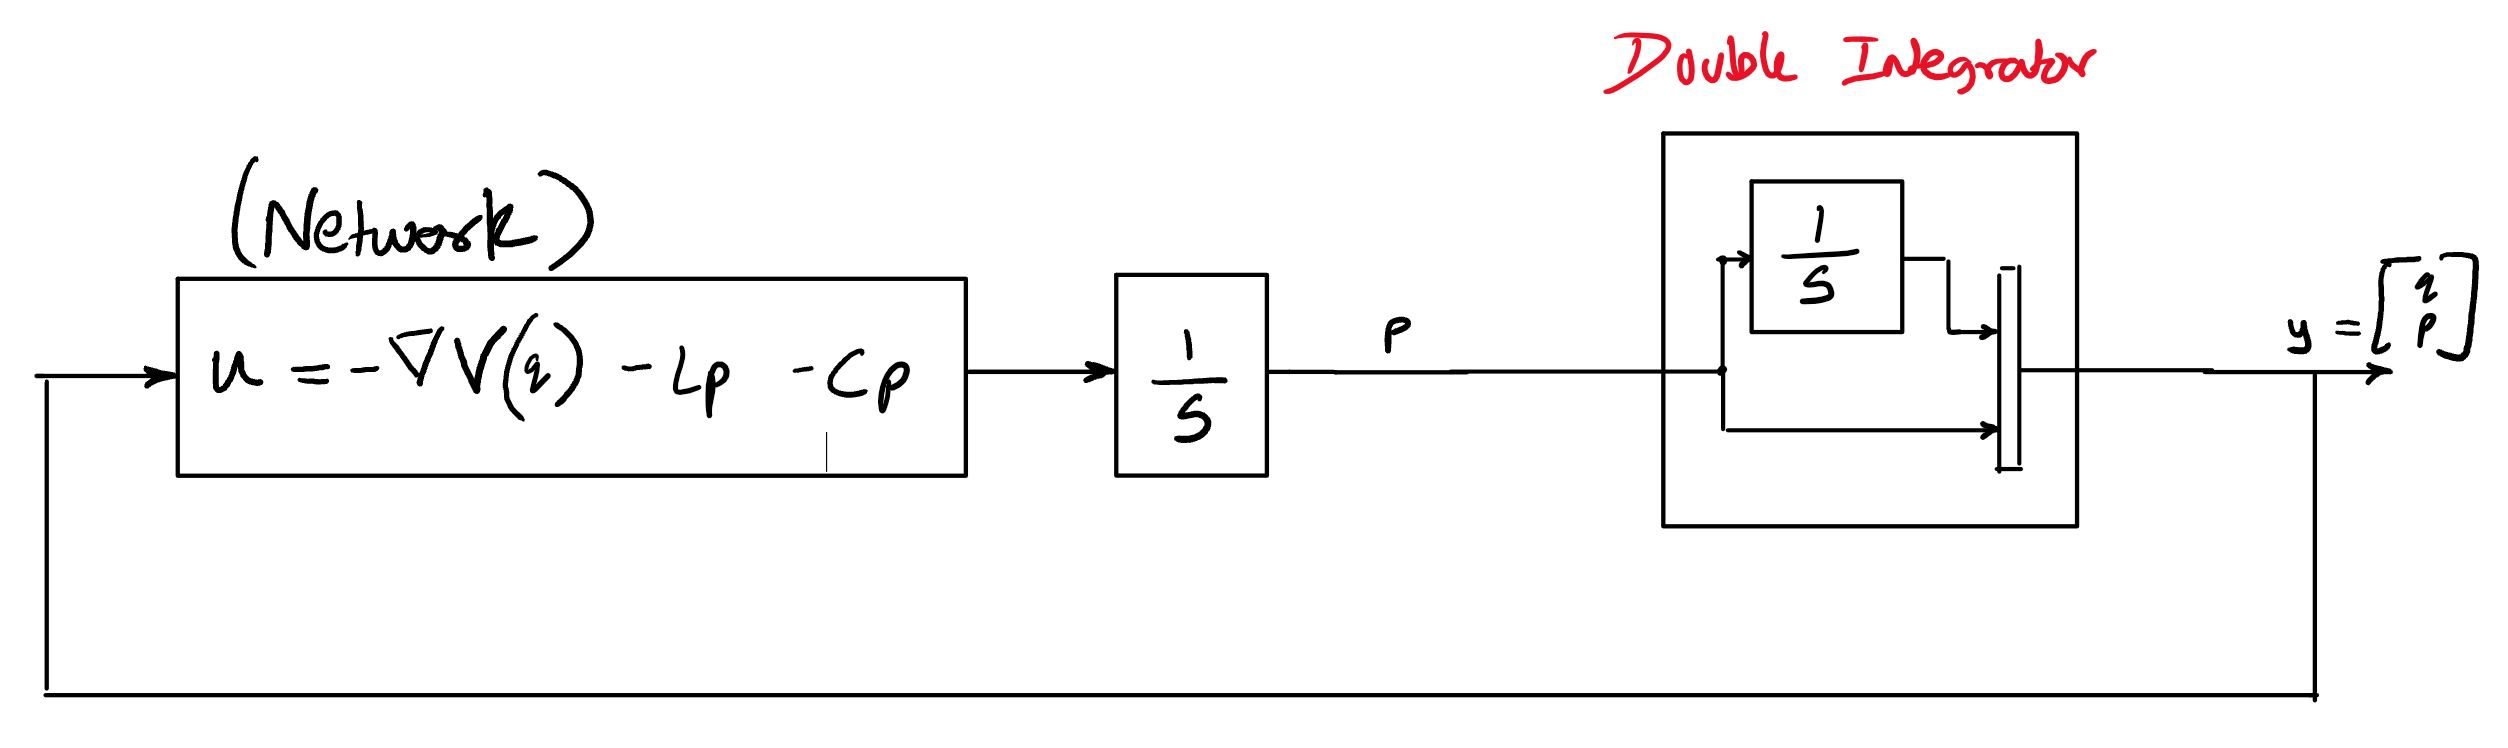
\includegraphics[scale=0.35]{figures/Coupled_flocking_double_integrators.jpg}	
		\label{fig:Coupled}
	\end{figure}
	\begin{itemize}
		\item Flocking of double integraor agents \footnote{Olfati Saber,2006}
		\item Stability analysis via LaSalle
	\end{itemize}
\end{frame}
%%%%%%%%%%%%%%%%%%%%%%%%%%%%%%%%%%%%%%%%%%%%%%%%%%%%%%%%%%%%%%%%%%%%%
%%%%%%%%%%%%%%%%%%%%%%%%%%%%%%%%%%%%%%%%%%%%%%%%%%%%%%%%%%%%%%%%%%%%%
\begin{frame}{Coupled architecture: Flocking}	
	\begin{figure}
		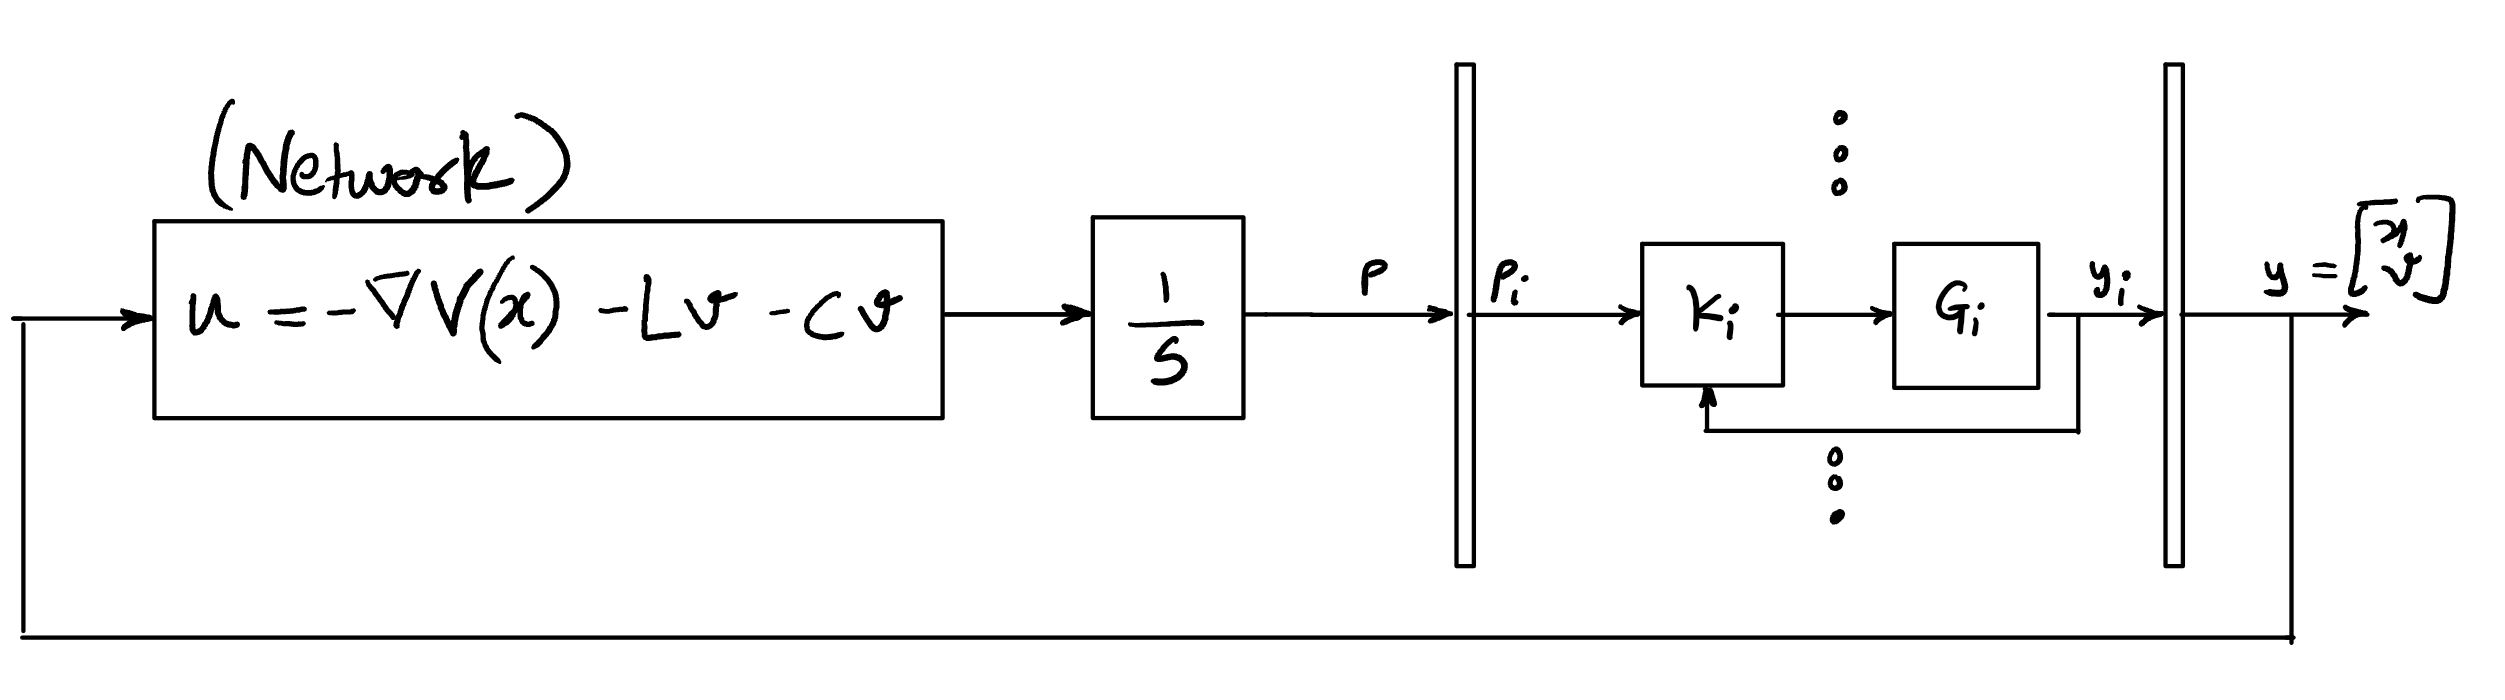
\includegraphics[scale=0.35]{figures/Coupled_flocking_quads.jpg}	
		\label{fig:Coupled}
	\end{figure}
	\begin{itemize}
		\item Flocking of quadrotors agents \footnote{Francis, 2016} but with fixed Laplacians
		\item Our experiments show that Quadrotors can be made to act like double integrators by well-tuned velocity controllers
	\end{itemize}
\end{frame}
%%%%%%%%%%%%%%%%%%%%%%%%%%%%%%%%%%%%%%%%%%%%%%%%%%%%%%%%%%%%%%%%%%%%%
%%%%%%%%%%%%%%%%%%%%%%%%%%%%%%%%%%%%%%%%%%%%%%%%%%%%%%%%%%%%%%%%%%%%%
\begin{frame}{Coupled architecture: Flocking and source-seeking \footnote{Datar, Paulsen, Werner, 2020}}
	\begin{figure}
		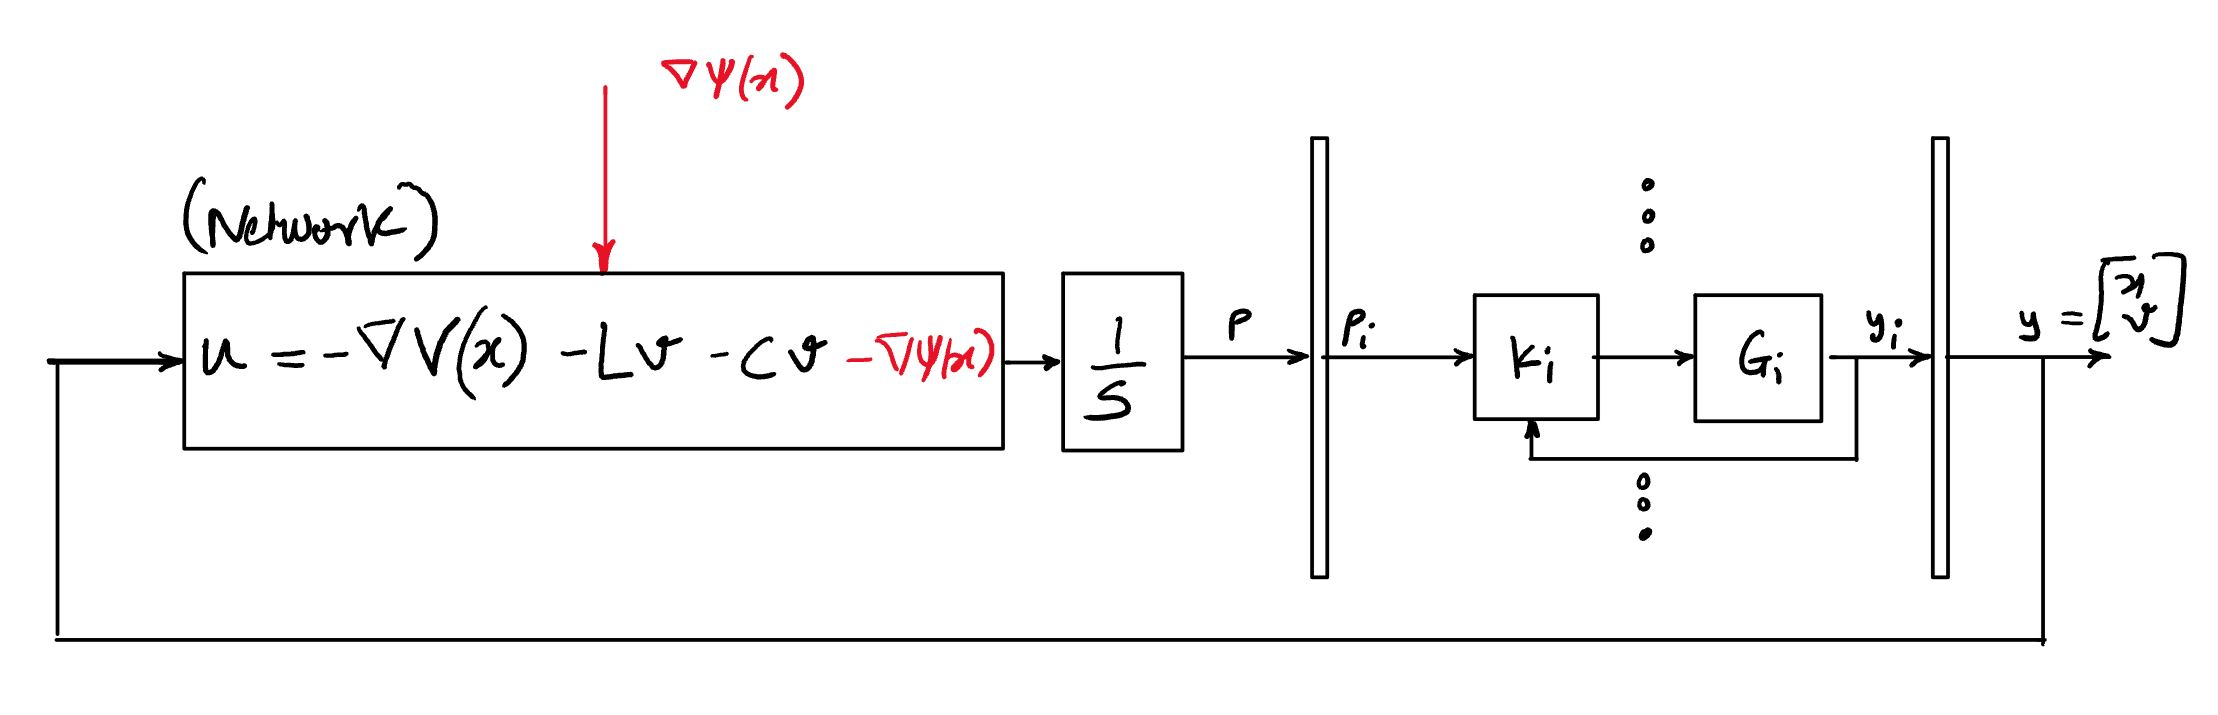
\includegraphics[scale=0.35]{figures/Coupled_flocking_quads_source_seek.jpg}	
		\label{fig:Coupled}
	\end{figure}	
	\begin{itemize}
		\item Forcing dynamics due to a scalar field
		\item Convergence analysis(Asymptotic stability) for double integrator agents
		\item Experiments by designing good local velocity controllers
	\end{itemize}
\end{frame}
%%%%%%%%%%%%%%%%%%%%%%%%%%%%%%%%%%%%%%%%%%%%%%%%%%%%%%%%%%%%%%%%%%%%%
%%%%%%%%%%%%%%%%%%%%%%%%%%%%%%%%%%%%%%%%%%%%%%%%%%%%%%%%%%%%%%%%%%%%%
\begin{frame}{Coupled architecture: Flocking and source-seeking with non-linear agents \footnote{Atallah, Datar, Werner, 2020}}	
	\begin{figure}
		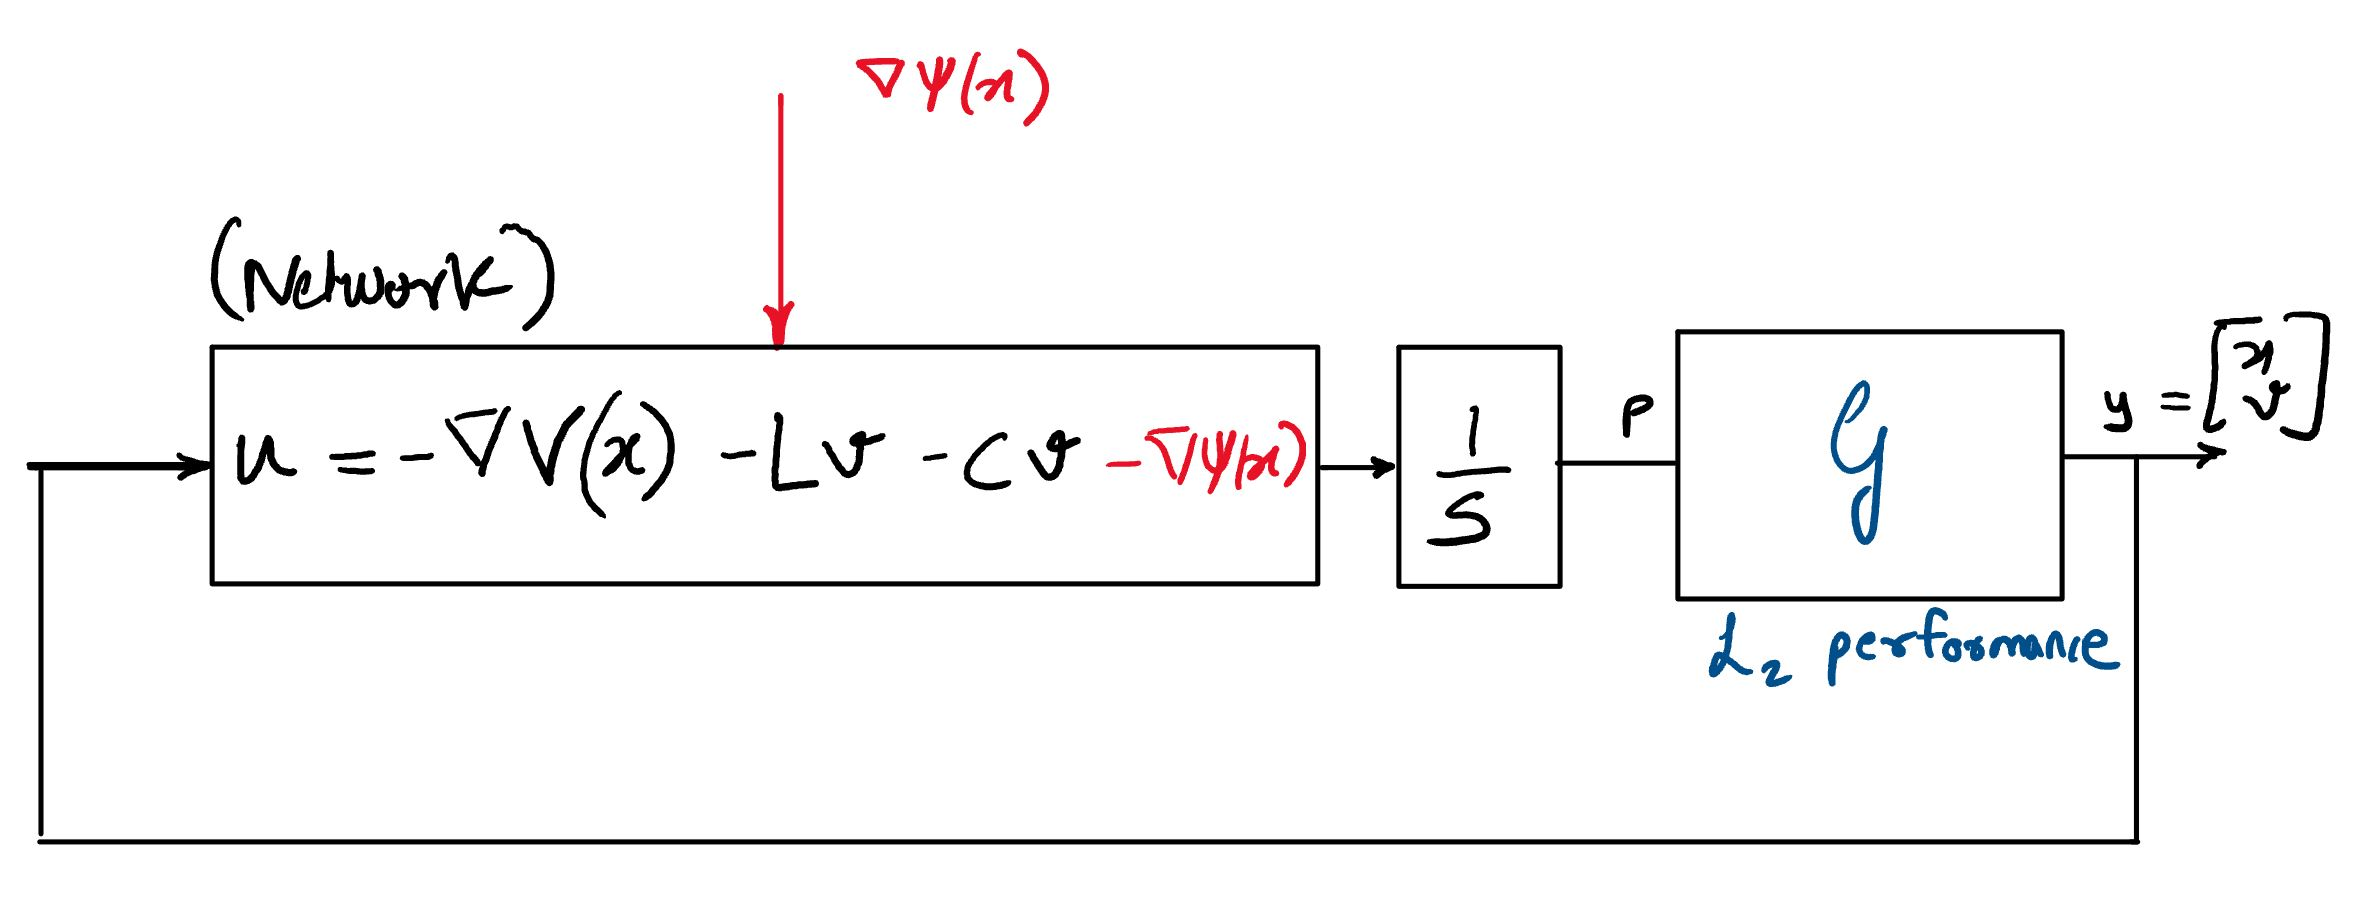
\includegraphics[scale=0.35]{figures/Coupled_flocking_gen_non_lin.JPG}	
		\label{fig:Coupled}
	\end{figure}
	\begin{itemize}
		\item From double integrators -> non-linear (LPV) agents
		\item Stability isL(not asymptotic) 
	\end{itemize}
\end{frame}
%%%%%%%%%%%%%%%%%%%%%%%%%%%%%%%%%%%%%%%%%%%%%%%%%%%%%%%%%%%%%%%%%%%%%
%%%%%%%%%%%%%%%%%%%%%%%%%%%%%%%%%%%%%%%%%%%%%%%%%%%%%%%%%%%%%%%%%%%%%
\begin{frame}{Coupled architecture: Some speculative ideas and open questions}	
	\begin{figure}
		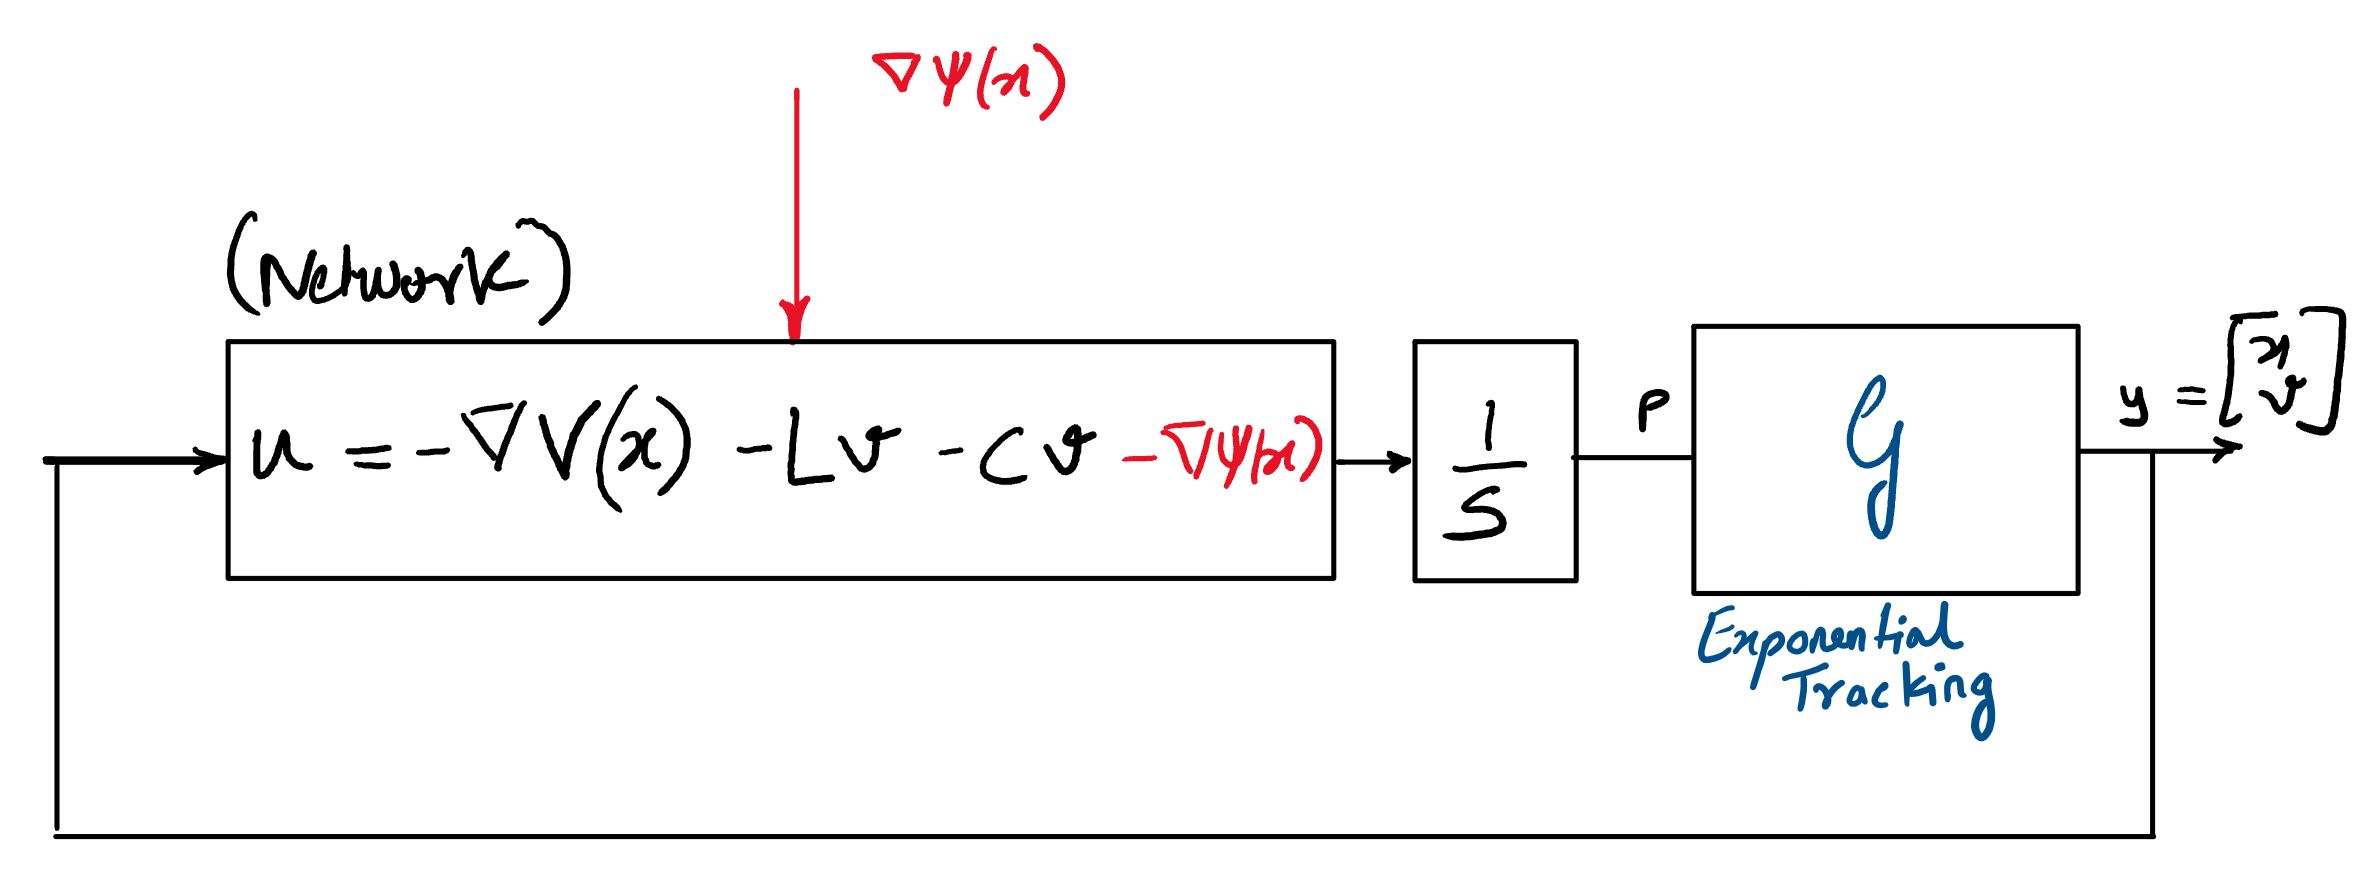
\includegraphics[scale=0.35]{figures/Coupled_flocking_gen_IQC.JPG}	
		\label{fig:Coupled}
	\end{figure}
	\begin{itemize}
		\item Use IQCs to obtain exponential convergence rates\footnote{Boczr,Recht,Lessard,Packard,2017} of local closed loops and use  singular perturbation argument such as in \footnote{Mesbahi and others,2018} 
	\end{itemize}
\end{frame}